\usetikzlibrary{calc,arrows,shapes,fit}

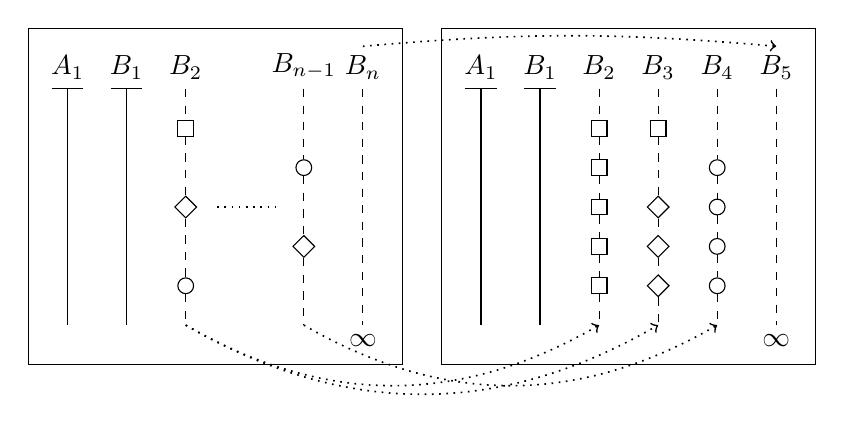
\begin{tikzpicture}
\tikzstyle{every label} = [font=\normalsize];
\tikzstyle{state} = [circle, inner sep=2pt, minimum size=2mm, draw=black, node distance=0.5cm]
\tikzstyle{hiddenstate} = [state, circle,inner sep=0pt,outer sep=0pt, minimum size=0pt, draw=gray]
\tikzstyle{topstate} = [hiddenstate, node distance=0.75cm]
\tikzstyle{state21} = [state, rectangle]
\tikzstyle{state22} = [state, diamond]
\tikzstyle{state23} = [state, regular polygon,circle]

%----------------------------------------------------------------------------------------------------------------------------

%T1_1
\node (t11_top) [topstate, label={[name=t11_top-label] $A_1$}] {};
\draw ($(t11_top)-(.2,0)$) -- ($(t11_top)+(.2,0)$);
\node (t11_1) [hiddenstate, below of=t11_top] {};
\node (t11_2) [hiddenstate, below of=t11_1] {};
\node (t11_3) [hiddenstate, below of=t11_2] {};
\node (t11_4) [hiddenstate, below of=t11_3] {};
\node (t11_5) [hiddenstate, below of=t11_4] {};
\node (t11_6) [hiddenstate, below of=t11_5] {};
\draw (t11_top) -- (t11_6);

%T2_1
\node (t21_top) [topstate, right of=t11_top, label={[name=t21_top-label] $B_1$}] {};
\draw ($(t21_top)-(.2,0)$) -- ($(t21_top)+(.2,0)$);
\node (t21_1) [hiddenstate, below of=t21_top] {};
\node (t21_2) [hiddenstate, below of=t21_1] {};
\node (t21_3) [hiddenstate, below of=t21_2] {};
\node (t21_4) [hiddenstate, below of=t21_3] {};
\node (t21_5) [hiddenstate, below of=t21_4] {};
\node (t21_6) [hiddenstate, below of=t21_5] {};
\draw (t21_top) -- (t21_6);


%T2_2
\node (t22_top) [topstate, right of=t21_top, label={[name=t22_top-label] $B_2$}] {};
\node (t22_1) [state21, below of=t22_top] {};
\node (t22_2) [hiddenstate, below of=t22_1] {};
\node (t22_3) [state22, below of=t22_2] {};
\node (t22_4) [hiddenstate, below of=t22_3] {};
\node (t22_5) [state23, below of=t22_4] {};
\node (t22_6) [hiddenstate, below of=t22_5] {};
\draw[dashed] (t22_top) -- (t22_1);
\draw[dashed] (t22_1) -- (t22_3);
\draw[dashed] (t22_3) -- (t22_5);
\draw[dashed] (t22_5) -- (t22_6);

% other processes placeholder
\node (t2i_top) [topstate, right of=t22_top] {};

% T_2_m
\node (t2m_top) [topstate, right of=t2i_top, label={[name=t2m_top-label] $B_{n-1}$}] {};
\node (t2m_1) [hiddenstate, below of=t2m_top] {};
\node (t2m_2) [state23, below of=t2m_1] {};
\node (t2m_3) [hiddenstate, below of=t2m_2] {};
\node (t2m_4) [state22, below of=t2m_3] {};
\node (t2m_5) [hiddenstate, below of=t2m_4] {};
\node (t2m_6) [hiddenstate, below of=t2m_5] {};
\draw[dashed] (t2m_top) -- (t2m_2);
\draw[dashed] (t2m_2) -- (t2m_4);
\draw[dashed] (t2m_4) -- (t2m_6);

% T_2_n
\node (t2n_top) [topstate, right of=t2m_top, label={[name=t2n_top-label] $B_n$}] {};
\node (t2n_1) [hiddenstate, below of=t2n_top] {};
\node (t2n_2) [hiddenstate, below of=t2n_1] {};
\node (t2n_3) [hiddenstate, below of=t2n_2] {};
\node (t2n_4) [hiddenstate, below of=t2n_3] {};
\node (t2n_5) [hiddenstate, below of=t2n_4] {};
\node (t2n_6) [hiddenstate, below of=t2n_5, label={[name=t2n_6-label]below:$\infty$}] {};
\draw[dashed] (t2n_top) -- (t2n_6);

%\draw[dashed] (t2n_2) -- (t2n_4);
%\draw[dashed] (t2n_4) -- (t2n_6);

\coordinate (t11_old-top) at (t11_top);
\coordinate (t11_old-bottom) at (t11_6);
\coordinate (t21_old-top) at (t21_top);
\coordinate (t21_old-bottom) at (t21_6);
\coordinate(t22_old-bottom) at (t22_6);
\coordinate (t2n_old-top) at (t2n_top);
%\coordinate(t2n_old-bottom) at (t2n_6);
\coordinate(t2m_old-bottom) at (t2m_6);
\coordinate(t2n_old-bottom) at ($(t2n_6-label)-(0,0.1)$);


% other processes line
\coordinate (t22_center) at ($(t22_3.center)$);
\coordinate (t2m_center) at ($(t2m_3.center)$);
\draw[dotted,semithick] ($(t22_center)+(0.4,0)$) to ($(t2m_center)-(0.3,0)$); % a bit cheating

% box
\node (box_outer) [draw=black, fit=(t11_top-label.center) (t2n_6), inner sep=0.5cm] {} ;
%\draw[solid] ($(t11_top-label)!0.5!(t21_top-label)+(0,0.5)$) to ($(t11_6)!0.5!(t21_6)-(0,0.5)$) ;
% \draw[solid] ($(t21_top-label)!0.5!(t22_top-label)+(0,0.5)$) to ($(t21_6)!0.5!(t22_6)-(0,0.5)$) ;



%----------------------------------------------------------------------------------------------------------------------------

%T1_1
\node (t11_top) [topstate, label={[name=t11_top-label] $A_1$}, right of=t2n_old-top, node distance=1.5cm] {};
\draw ($(t11_top)-(.2,0)$) -- ($(t11_top)+(.2,0)$);
\node (t11_1) [hiddenstate, below of=t11_top] {};
\node (t11_2) [hiddenstate, below of=t11_1] {};
\node (t11_3) [hiddenstate, below of=t11_2] {};
\node (t11_4) [hiddenstate, below of=t11_3] {};
\node (t11_5) [hiddenstate, below of=t11_4] {};
\node (t11_6) [hiddenstate, below of=t11_5] {};
\draw (t11_top) -- (t11_6);

%T2_1
\node (t21_top) [topstate, right of=t11_top, label={[name=t21_top-label] $B_1$}] {};
\draw ($(t21_top)-(.2,0)$) -- ($(t21_top)+(.2,0)$);
\node (t21_1) [hiddenstate, below of=t21_top] {};
\node (t21_2) [hiddenstate, below of=t21_1] {};
\node (t21_3) [hiddenstate, below of=t21_2] {};
\node (t21_4) [hiddenstate, below of=t21_3] {};
\node (t21_5) [hiddenstate, below of=t21_4] {};
\node (t21_6) [hiddenstate, below of=t21_5] {};
\draw (t21_top) -- (t21_6);


%T2_2
\node (t22_top) [topstate, right of=t21_top, label={[name=t22_top-label] $B_2$}] {};
\node (t22_1) [state21, below of=t22_top] {};
\node (t22_2) [state21, below of=t22_1] {};
\node (t22_3) [state21, below of=t22_2] {};
\node (t22_4) [state21, below of=t22_3] {};
\node (t22_5) [state21, below of=t22_4] {};
\node (t22_6) [hiddenstate, below of=t22_5] {};
\draw[dashed] (t22_top) -- (t22_1);
\draw[dashed] (t22_1) -- (t22_2);
\draw[dashed] (t22_2) -- (t22_3);
\draw[dashed] (t22_3) -- (t22_4);
\draw[dashed] (t22_4) -- (t22_5);
\draw[dashed] (t22_5) -- (t22_6);

% other processes placeholder
\node (t2i_top) [topstate, right of=t22_top] {};

% T_2_3
\node (t23_top) [topstate, right of=t22_top, label={[name=t23_top-label] $B_3$}] {};
\node (t23_1) [state21, below of=t23_top] {};
\node (t23_2) [hiddenstate, below of=t23_1] {};
\node (t23_3) [state22, below of=t23_2] {};
\node (t23_4) [state22, below of=t23_3] {};
\node (t23_5) [state22, below of=t23_4] {};
\node (t23_6) [hiddenstate, below of=t23_5] {};
\draw[dashed] (t23_top) -- (t23_1);
\draw[dashed] (t23_1) -- (t23_3);
\draw[dashed] (t23_3) -- (t23_4);
\draw[dashed] (t23_4) -- (t23_5);
\draw[dashed] (t23_5) -- (t23_6);


% T_2_4
\node (t24_top) [topstate, right of=t23_top, label={[name=t24_top-label] $B_4$}] {};
\node (t24_1) [hiddenstate, below of=t24_top] {};
\node (t24_2) [state23, below of=t24_1] {};
\node (t24_3) [state23, below of=t24_2] {};
\node (t24_4) [state23, below of=t24_3] {};
\node (t24_5) [state23, below of=t24_4] {};
\node (t24_6) [hiddenstate, below of=t24_5] {};
\draw[dashed] (t24_top) -- (t24_2);
\draw[dashed] (t24_2) -- (t24_3);
\draw[dashed] (t24_3) -- (t24_4);
\draw[dashed] (t24_4) -- (t24_5);
\draw[dashed] (t24_5) -- (t24_6);

% T_2_5
\node (t25_top) [topstate, right of=t24_top, label={[name=t25_top-label] $B_5$}] {};
\node (t25_1) [hiddenstate, below of=t25_top] {};
\node (t25_2) [hiddenstate, below of=t25_1] {};
\node (t25_3) [hiddenstate, below of=t25_2] {};
\node (t25_4) [hiddenstate, below of=t25_3] {};
\node (t25_5) [hiddenstate, below of=t25_4] {};
\node (t25_6) [hiddenstate, below of=t25_5, label={[name=t25_6-label]below:$\infty$}] {};
\draw[dashed] (t25_top) -- (t25_6);


\coordinate (t11_new-top) at (t11_top);
\coordinate (t11_new-bottom) at (t11_6);
\coordinate (t21_new-top) at (t21_top);
\coordinate (t21_new-bottom) at (t21_6);
\coordinate (t22_new-top) at (t22_top);
\coordinate (t22_new-bottom) at (t22_6);
\coordinate(t23_new-bottom) at (t23_6);
\coordinate(t24_new-bottom) at (t24_6);
%\coordinate(t25_new-bottom) at (t25_6);
\coordinate(t25_new-bottom) at ($(t25_6-label)-(0,0.1)$);

% box
\node (box_outer) [draw=black, fit=(t11_top-label.center) (t25_6), inner sep=0.5cm] {} ;
%\draw[solid] ($(t11_top-label)!0.5!(t21_top-label)+(0,0.5)$) to ($(t11_6)!0.5!(t21_6)-(0,0.5)$) ;
% \draw[solid] ($(t21_top-label)!0.5!(t22_top-label)+(0,0.5)$) to ($(t21_6)!0.5!(t22_6)-(0,0.5)$) ;

\draw[->, bend right, dotted,semithick] (t22_old-bottom) to (t22_new-bottom);
\draw[->, bend right, dotted,semithick] (t22_old-bottom) to (t23_new-bottom);
\draw[->, bend right, dotted,semithick] (t2m_old-bottom) to (t24_new-bottom);
%\draw[->, bend right, dotted,semithick] (t2n_old-bottom) to (t25_new-bottom);
%\draw[->, bend left, dotted,semithick] (t2m_top-label.north) to (t24_top-label.north);
\draw[->, bend left=5, dotted,semithick] (t2n_top-label.north) to (t25_top-label.north);


\end{tikzpicture}